% Figure from MATH 591 notes, section 67. Added, not from lecture: TM = R x R; a field is a graph, the lift of c(t) = t^2 - 1 meets T_0M twice.
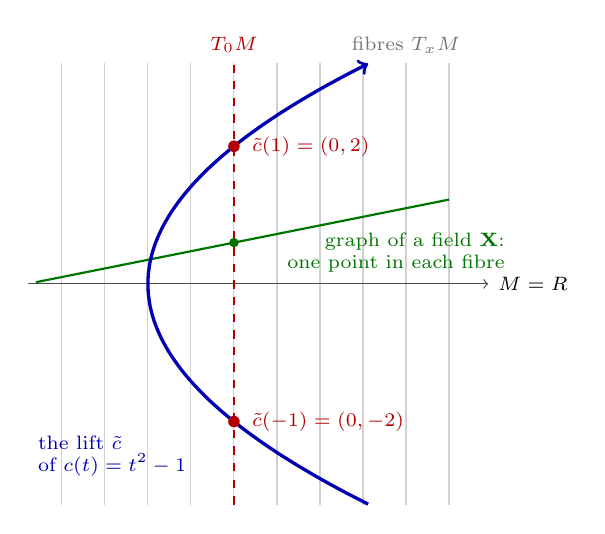
\begin{tikzpicture}[scale=0.95]
\foreach \x in {-2,-1.5,...,2.5} { \draw[black!18] ({1.15*\x},-2.95) -- ({1.15*\x},2.95); }
\draw[->, black!70] (-2.75,0) -- (3.4,0) node[right, font=\scriptsize, text=black] {$M = \mathbb{R}$};
\node[font=\scriptsize, black!55, anchor=south] at (2.3,2.95) {fibres $T_xM$};
\draw[green!45!black, thick] (-2.645,0.023) -- (2.875,1.127);
\node[green!45!black, font=\scriptsize, align=right, anchor=east] at (3.75,0.42) {graph of a field $\mathbf{X}$:\\ one point in each fibre};
\draw[blue!70!black, very thick, ->] plot[smooth] coordinates {(1.794,-2.944) (1.649,-2.870) (1.507,-2.797) (1.369,-2.723) (1.235,-2.650) (1.104,-2.576) (0.977,-2.502) (0.854,-2.429) (0.734,-2.355) (0.618,-2.282) (0.506,-2.208) (0.397,-2.134) (0.293,-2.061) (0.191,-1.987) (0.094,-1.914) (0.000,-1.840) (-0.090,-1.766) (-0.177,-1.693) (-0.259,-1.619) (-0.339,-1.546) (-0.414,-1.472) (-0.486,-1.398) (-0.554,-1.325) (-0.618,-1.251) (-0.679,-1.178) (-0.736,-1.104) (-0.789,-1.030) (-0.839,-0.957) (-0.885,-0.883) (-0.927,-0.810) (-0.966,-0.736) (-1.001,-0.662) (-1.032,-0.589) (-1.060,-0.515) (-1.084,-0.442) (-1.104,-0.368) (-1.121,-0.294) (-1.133,-0.221) (-1.143,-0.147) (-1.148,-0.074) (-1.150,0.000) (-1.148,0.074) (-1.143,0.147) (-1.133,0.221) (-1.121,0.294) (-1.104,0.368) (-1.084,0.442) (-1.060,0.515) (-1.032,0.589) (-1.001,0.662) (-0.966,0.736) (-0.927,0.810) (-0.885,0.883) (-0.839,0.957) (-0.789,1.030) (-0.736,1.104) (-0.679,1.178) (-0.618,1.251) (-0.554,1.325) (-0.486,1.398) (-0.414,1.472) (-0.339,1.546) (-0.259,1.619) (-0.177,1.693) (-0.090,1.766) (0.000,1.840) (0.094,1.914) (0.191,1.987) (0.293,2.061) (0.397,2.134) (0.506,2.208) (0.618,2.282) (0.734,2.355) (0.854,2.429) (0.977,2.502) (1.104,2.576) (1.235,2.650) (1.369,2.723) (1.507,2.797) (1.649,2.870) (1.794,2.944)};
\draw[red!70!black, thick, dashed] (0,-2.95) -- (0,2.95) node[above, font=\scriptsize] {$T_0M$};
\fill[green!45!black] (0,0.552) circle (1.8pt);
\fill[red!70!black] (0,1.840) circle (2.2pt) node[right=3pt, font=\scriptsize] {$\tilde c(1) = (0, 2)$};
\fill[red!70!black] (0,-1.840) circle (2.2pt) node[right=3pt, font=\scriptsize] {$\tilde c(-1) = (0, -2)$};
\node[blue!70!black, font=\scriptsize, align=left, anchor=west] at (-2.75,-2.3) {the lift $\tilde c$\\ of $c(t) = t^2 - 1$};
\end{tikzpicture}
